\section{Aplicação Desenvolvida}
Para a segunda entrega do aplicativo, foram desenvolvidos os seguintes requisitos já elicitados na primeira entrega:
\begin{itemize}
    \item Eu, como motorista, gostaria de me cadastrar no sistema para ter acesso ao login;
    \item Eu, como motorista, gostaria de logar no sistema para utilizar as funcionalidades do mesmo;
    \item Eu, como motorista, gostaria de ver os postos dentro de uma rota para facilitar a minha escolha de posto;
    \item Eu, como motorista, gostaria de avaliar o posto onde eu abasteci para atribuir uma qualidade ao mesmo;
    \item Eu, como motorista, gostaria de informar se estou ou não abastecendo no posto para contribuir com os dados coletados pelo aplicativo;
    \item Eu, como motorista, gostaria de ver uma lista com todos os postos boicotados para me programar com antecedência em onde abastecer;
    \item Eu, como motorista, gostaria de saber quando eu estou em um posto de combustíveis para interagir com o mesmo;
    \item Eu, como motorista, gostaria de editar o meu cadastro para manter minhas informações atualizadas;
    \item Eu, como motorista, gostaria de registrar o preço de combustíveis, álcool ou diesel do posto onde eu me encontro para ele sempre estar com o preço correto;
    \item Eu, como desenvolvedor, desejo mapear os postos de combustíveis para que sejam tratados no sistema;
    \item Eu, como motorista, gostaria de editar o meu cadastro para manter minhas informações atualizadas;
    \item Eu, como motorista, gostaria de ver as informações do posto onde eu estou, para saber se quero abastecer nele ou não.
\end{itemize}

Além desses requisitos, foram elicitados os seguintes novos itens que se mostraram imprescindíveis para a aplicação:

\begin{itemize}
    \item Eu, como administrador, gostaria de entrar no sistema para ajustar configurações básicas do sistema;
    \item Eu, como administrador, gostaria de adicionar as bandeiras dos postos para facilitar a identificação pelo usuário;
    \item Eu, como administrador, gostaria de alterar as informações dos postos cadastrados para garantir a verossimilhança dos dados vindos de fontes externas ao sistema;
    \item Eu, como motorista, gostaria de visualizar um gráfico contendo os gastos mensais com combustível para controlar melhor o meu orçamento;
    \item Eu, como motorista, gostaria de visualizar um histórico de postos onde passei para controlar melhor os meus gastos.
\end{itemize}

COLOCAR PRINTS DE ALGUMAS TELAS ENTRE ALGUNS ITENS

As funcionalidades de administrador se mostraram imprescindíveis para facilitar a identificação dos postos de combustíveis pelo usuário através de ícones nos postos de gasolina indicando as bandeiras dos postos. Além disso, como a primeira versão do aplicativo que vai para a Play Store não irá possuir as funcionalidades que irão garantir a qualidade dos dados de preços dos combustíveis, mostrou-se importante ser possível editar os dados manualmente de forma mais prática. Viu-se também a importância de manter um controle na aplicação no que tange a controle de gastos do motorista e como isso age como um diferencial dos aplicativos atuais. 

No Anexo \ref{chap:telas} encontram-se algumas telas da aplicação desenvolvida.

\subsection{Método de decisão de postos boicotados}
Toda semana, serão selecionados postos onde os usuários serão incentivados a não abastecer. Para decidir quais postos serão boicotados, o Guimifiu tem duas estratégias principais: a \textbf{Lista Comum} e o \textbf{Boicote por Bandeiras}. A lista comum escolhe os postos com pior qualidade geral e que não tenham sido boicotados recentemente e cria uma lista inicial. A qualidade geral de um posto é determinada pela média ponderada de estrelas do posto e pelo preço dos combustíveis considerando o preço de todos os postos. O preço cada combustível tem peso 2 e o inverso da quantidade de estrelas tem peso 1. O cálculo é realizado com a seguinte equação:

\begin{equation}
\label{Equação para cálculo de qualidade geral do Combustível}
	QG = \frac{1*QE}{2*(PG + PA + PD)}
\end{equation}

Sendo que QG é a Qualidade Geral do posto, PG, PA e PD são os preços de Gasolina, Álcool e Diesel, respectivamente e, por fim, QE é a Quantidade de Estrelas.

A lista inicial é montada e depois é verificado se não existem muitos postos perto demais sendo boicotados para não deixar o usuário com poucas opções de locais para abastecimento. Essa verificação é feita através de grafos. Os nós dos grafos são os postos de combustíveis e as arestas são as distâncias entre os todos postos que não sejam maiores que 10 quilômetros. Com este grafo, em cada nó da lista inicial é verificado se os nós adjacentes são todos postos que estão na lista inicial. Em caso positivo, o nó é removido da lista, caso contrário o nó é mantido. Os nós restantes compõem a lista final de postos boicotados, denominada \textbf{Lista Comum}. Na Figura a seguir, considerando que os pontos vermelhos são nós da lista inicial e os pontos azuis são o resto dos postos, após a verificação, os pontos vermelhos virariam azuis como na próxima figura.

\begin{figure}[H]
    \centering
    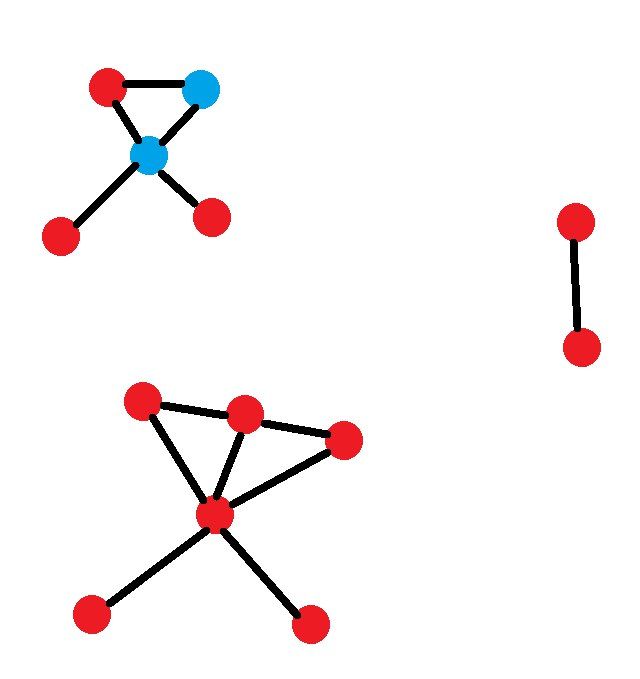
\includegraphics[scale=0.5]{figuras/listainicial.jpg}
    \caption[Grafo com Lista Inicial de Postos Boicotados]{Grafo com Lista Inicial de Postos Boicotados. Fonte: autores}
    \label{img:listainicial}
\end{figure}

\begin{figure}[H]
    \centering
    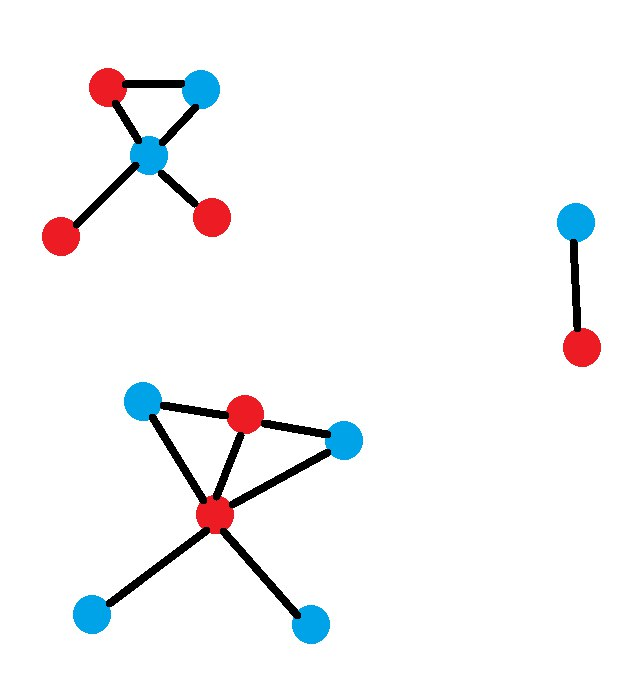
\includegraphics[scale=0.5]{figuras/listacomum.jpg}
    \caption[Grafo com Lista Comum de Postos Boicotados]{Grafo com Lista Comum de Postos Boicotados. Fonte: autores}
    \label{img:listacomum}
\end{figure}

O \textit{Boicote por Bandeiras} escolhe uma bandeira e todos os postos dessa bandeira são colocados na lista de boicotados, independentemente da distância entre eles, colocando o prejuízo do boicote menos nos postos e mais na bandeira. Os dois tipos de boicote são exclusivos, ou seja, os dois não ocorrem no mesmo período. A estratégia de boicote é escolhida pela equipe de desenvolvimento.  

\subsection{Testes Automatizados}

Foram feitos testes de integração e unitários para garantir o funcionamento dos métodos do código fonte e da integração da aplicação \textit{mobile} com a API.

Foi encontrada uma certa dificuldade pra realizar os testes unitários no Ionic, uma vez que não há muitos exemplos que de fato funcionam e uma documentação do próprio \textit{framework} sobre o assunto.

O código de testes pode ser encontrado no repositório da aplicação no GitHub (https://github.com/Guimifiu/guimifiu-app). Um exemplo de teste unitário e um de teste de integração está disponível no Anexo \ref{chap:testes}.

\subsection{Métricas de Código fonte}

Como citado no \autoref{chap:met}, foram utilizadas as ferramentas CodeClimate e Rubocop. Além de medir a complexidade no Rubocop, foi feita na integração contínua um relatório de métricas pela ferramenta que impede que a \textit{build} passe caso a complexidade seja maior do que 6, que é o padrão de complexidade ciclomática máxima aceitável.

A Figura \ref{img:rubocop} mostra o resultado da análise feita pelo Rubocop. O arquivo de configuração utilizado para a análise pode ser encontrado no endereço do Github do  \citeonline{rubocop-guimifiu}.

\begin{figure}[H]
    \centering
    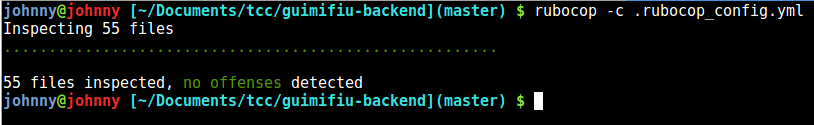
\includegraphics[scale=0.5]{figuras/rubocop.png}
    \caption[Relatório de análise estática do Rubocop]{Relatório de análise estática do Rubocop. Fonte: autores}
    \label{img:rubocop}
\end{figure}

A Figura \ref{img:codeclimate} mostra o resultado das análises realizado pelo \href{https://codeclimate.com/github/Guimifiu/guimifiu-backend/}{CodeClimate}. 

\begin{figure}[H]
    \centering
    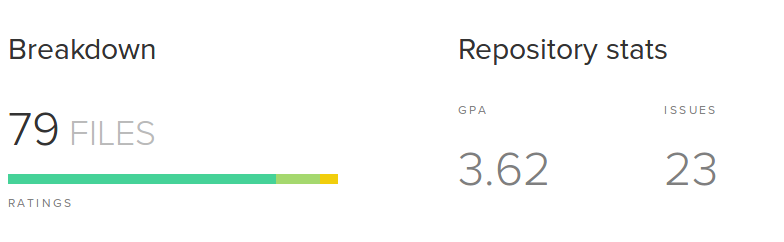
\includegraphics[scale=0.5]{figuras/codeclimate.png}
    \caption[Relatório de análise estática do CodeClimate]{Relatório de análise estática do CodeClimate. Fonte: autores}
    \label{img:codeclimate}
\end{figure}

Seis das sete \textit{issues} encontradas foram por motivo do CodeClimate utilizar um parser com uma versão menor do que a versão do Ruby utilizada pela equipe, enquanto a última foi uma duplicação de código que será tratada durante a segunda parte do trabalho.


\subsection{Integração e Entrega Contínua}
Há três tipos de ambientes no desenvolvimento desta aplicação: \textit{development}, \textit{staging} e \textit{production}. O ambiente de \textit{development} ou desenvolvimento, é o ambiente local de cada desenvolvedor, \textit{staging} ou pré produção é um ambiente para serem realizados testes beta e \textit{production} ou produção é o ambiente final onde a aplicação será de fato utilizada pelos usuários.

Na API a integração contínua é feita com a ferramenta TravisCI. Onde, se um \textit{pull request} é aceito na \textit{branch} \textit{staging}, o Travis executa toda a suíte de testes para ver se algum deles pode ter resultado em falha, caso todos passem, ele verifica se todas as métricas definidas pelo Rubocop estão de acordo com o padrão definido. Caso todas as métricas passem, a build de pré produção é criada, o Travis envia as informações de cobertura de testes para o Coveralls, as informações de métricas para o Code Climate e logo em seguida realiza o \textit{deploy} no ambiente de pré produção no Heroku.

Caso um \textit{pull request} seja aceito na \textit{branch} \textit{master} todo o processo será o mesmo, com exceção que o \textit{deploy} irá ocorrer no ambiente de produção no Heroku.

A figura \ref{img:integracao_deploy_continuo_api} ilustra o processo de integração e deploy contínuo feito na API.

\begin{figure}[H]
    \centering
    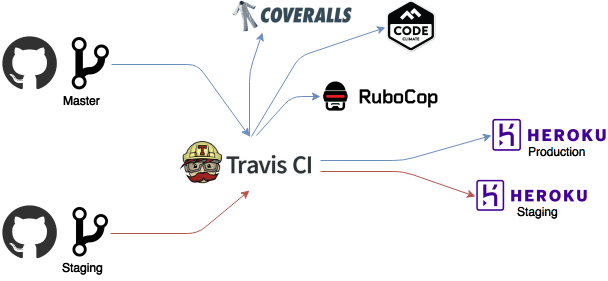
\includegraphics[scale=0.5]{figuras/api_ci.png}
    \caption[Integração e deploy contínuo API]{Integração e deploy contínuo API.}
    \label{img:integracao_deploy_continuo_api}
\end{figure}

No aplicativo, foi planejada a integração e o deploy contínuo para ocorrer da seguinte forma:

\begin{figure}[H]
    \centering
    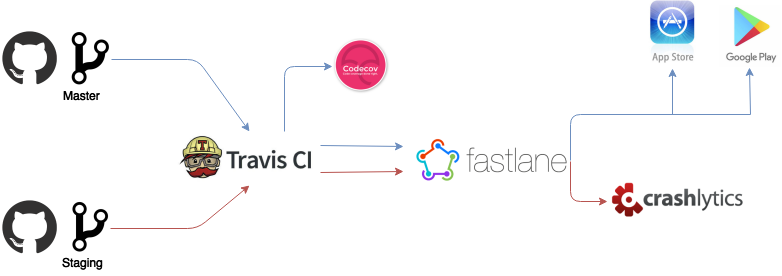
\includegraphics[scale=0.5]{figuras/ci_should_be.png}
    \caption[Integração e deploy contínuo planejado para o APP]{Integração e deploy contínuo planejado para o APP}
    \label{img:integracao_deploy_continuo_planejado_app}
\end{figure}

Se um pull request \textit{pull request} é aceito na \textit{branch} \textit{master}, o Travis irá realizar toda a suíte de testes, caso todos passem enviará as informações de cobertura para o
Codecov e através do Fastlane realizará o deploy do aplicativo tanto na Play Store quanto na App Store. E caso um \textit{pull request} é aceito na \textit{branch} \textit{staging}, todo o processo é repetido, com exceção
que não é realizado o deploy do aplicativo nas lojas e sim no Crashlytics, que irá criar a versão beta do aplicativo e enviará por email para os emails configurados previamente.

Uma vez que o aplicativo ainda não chegou ao estágio de deploy nas lojas, o planejamento para a primeira entrega é só até o deploy beta, como mostrado na figura \ref{img:integracao_deploy_continuo_planejado_primeira_entrega}:

\begin{figure}[H]
    \centering
    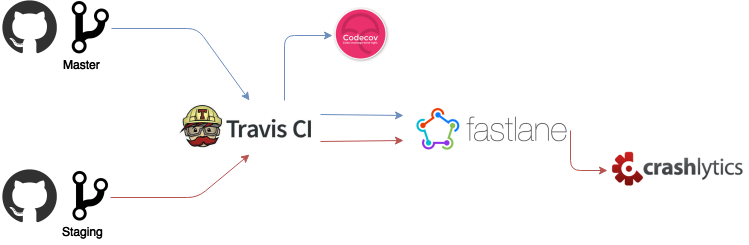
\includegraphics[scale=0.5]{figuras/ci_as_is.png}
    \caption[Integração e deploy contínuo planejado para o APP]{Integração e deploy contínuo planejado para a primeira entrega}
    \label{img:integracao_deploy_continuo_planejado_primeira_entrega}
\end{figure}

Porém não foi possível fazer com que o deploy contínuo aconteça logo após a integração contínua, um desafio causado por escolher desenvolvimento híbridos de aplicativo.
Uma vez que o código versionado do aplicativo é o mesmo código para a plataforma Android e iOS, e após realizar a build desse código é gerado códigos em cada plataforma (não versionados),
a ferramenta de integração contínua não consegue ter acesso aos códigos de cada plataforma para realizar os devidos deploys. Sendo assim, o deploy contínuo está acontecendo manualmente
por enquanto que nenhuma solução ainda foi encontrada, através do comando:

\begin{lstlisting}[language=bash]
  $ fastlane beta
\end{lstlisting}

Sendo assim, a figura \ref{img:integracao_deploy_continuo_atual} ilustra como está funcionando a integração e o deploy contínuo do aplicativo até o presente momento.

\begin{figure}[H]
    \centering
    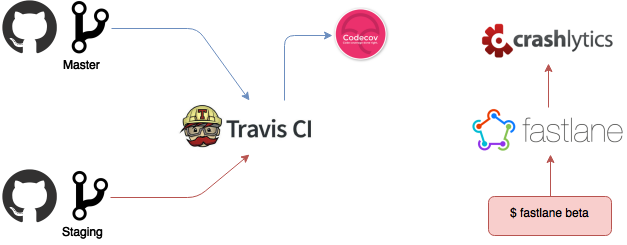
\includegraphics[scale=0.5]{figuras/ci_currently.png}
    \caption[Integração e deploy contínuo atual]{Integração e deploy contínuo atual}
    \label{img:integracao_deploy_continuo_atual}
\end{figure}


